\section{Experimentellt genomförande}
\label{sec:exper}
För att kunna analysera reaktionshastigheten behöver ni kunna följa
reaktionens gång som funktion av tid. Till ert förfogande kommer ni ha en
s.k. ``stopped-flow''-utrustning (se \cref{fig:stopped-flow}).

\begin{figure}[center]
  \centering
  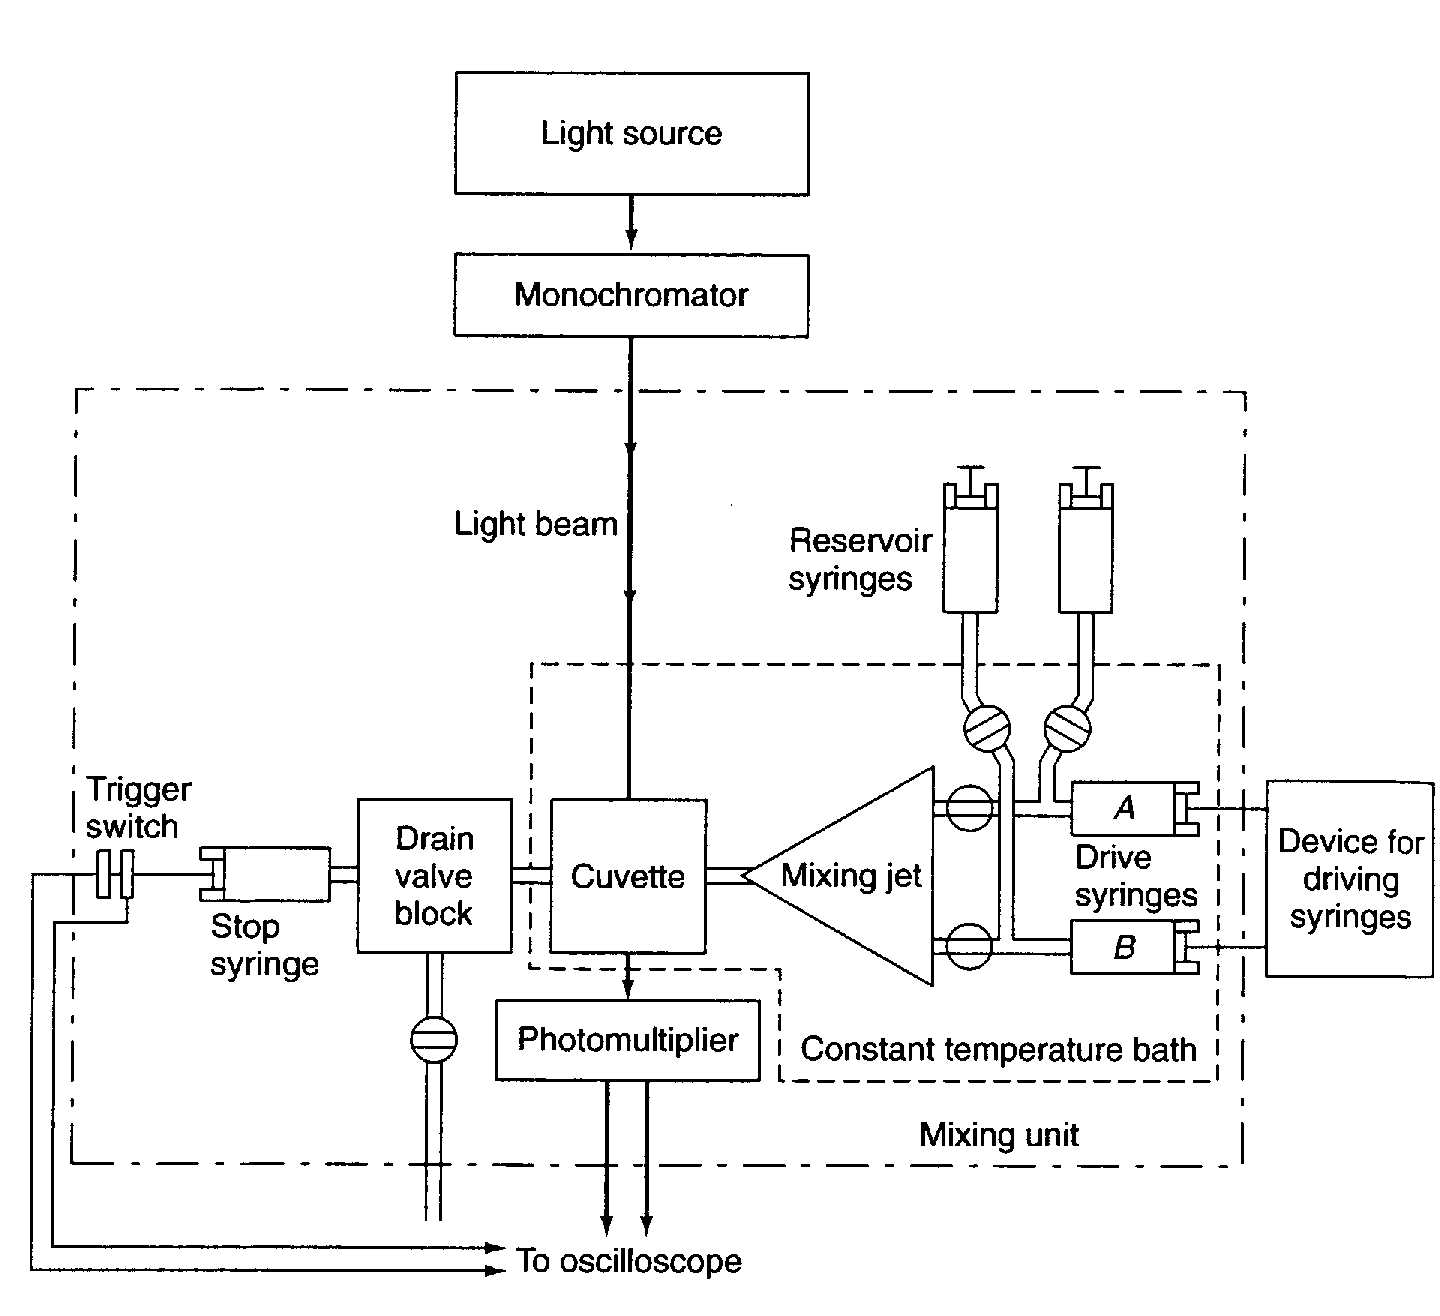
\includegraphics[scale=0.2]{fig/stopped_flow.png}
  \caption{Schematisk representation av stopped-flow utrustning}
  \label{fig:stopped-flow}
\end{figure}

Blandkammaren är termostaterad med hjälp av vattenbad som ni själva får
välja temperatur för. Ni kan börja era försök vid
rumstemperatur, temperaturintervallet ni kan arbeta inom styrs av
temperaturen av kallvattnet i husets ledningar (säg \SI{12}{\celsius})
och vattenbadets övre gräns (säg \SI{50}{\celsius}). 

Kyvettens längd är \SI{1}{\centi\metre} (vilket
tillsammans med extinktionskoefficienten  är något ni har nytta av att
veta när ni väljer koncentrationsintervall för era reaktantlösningar).

Istället för ett oscilloskåp kommer ni ha en dator med ett interface
skrivet i LabView. Handhavandet av programmet är beskrivet i
\cref{sec:handhavande}. Från varje försök kommer ni att erhålla dataserier med
absorbans som funktion av tid vid en våglängd som ni själva väljer. Dessa
tidsserier kommer sparas i form av textfiler som ni sparar på USB minne
som ni själva tar med er till labb.

\subsection{Stamlösningar}
För att bereda era reaktantlösningar kommer ni ha tillgång till följande
stamlösningar:

\begin{itemize}
\item \SI{1}{\Molar} \ce{NaClO4}
\item \SI{1}{\Molar} \ce{HClO4}
\item \SI{100}{\milli\Molar} \ce{KSCN}
\item \SI{100}{\milli\Molar} \ce{Fe(NO3)3}
\end{itemize}

\subsection{Handhavande}
\label{sec:handhavande}
Nedan finner ni en instruktion för handhavandet av
laborationsutrustningen.

\subsubsection{Förberedelser}
\begin{itemize}
\item Tänd lampan minst 5 minuter innan mätningarna.
\item Kontrollera att vattennivån i termostaten är tillräckligt hög.
Starta termostat och lägg i extern termometer.
\item Kontrollera att kylvattnet är på med hjälp av den röda flödesmätaren.
\item Sätt på kranvattnet.
\item Ställ in och invänta rätt temperatur
OBS! Vid alla mätningar och kalibreringar ska ``Stop'' vara nedtryckt på ``Start/Stop
Acquisition``. Om programmet stängs av måste kalibreringen (med dest. vatten) göras om,
tryck därför aldrig på ``Exit''. Undvik att luftbubblor kommer in i kyvetten.
\end{itemize}
\subsubsection{Kalibrering}
\begin{itemize}
\item Ställ ``Integration time'' till 2 ms.
\item Blockera strålgången med metallplåten. Tryck på ``Dark''. Ta bort metallplåten.
\item Injicera destillerat vatten. Tryck på ``Ref''.
\item Kontrollera att transmittansen och absorptionen ser ut som de bör.
\item Byt sprutor och injicera tillräckligt med reaktantlösning så att komplexet bildas i kyvetten.
\item Gå in i absorptionstfönstret och bestäm vid vilken våglängd mätningarna ska göras genom
att välja ``Peak'' i Integral/peak-menyn och ``drag-drop'':a den
vertikala linjen där ni vill mäta. Beakta att det viktiga måttet vid val
av våglängd är förhållandet mellan signal och brus (``signal-to-noise-ratio'').
\end{itemize}
\subsubsection{Mätning}
\begin{itemize}
\item Gå in på fliken ``Time mode''.
\item Välj ``As fast as possible'', ``Save to file'' och ``Use a trigger''.
\item Tryck på ``Start'' så att den gröna lampan lyser (triggern aktiveras).
\item Vinkla samtliga T-kranar nedåt.
\item Injicera snabbt in ny reaktantlösning. Håll kvar greppet i 4 sekunder.
\item Välj alltid ``Replace'' när frågerutan dyker upp (se till att
  kopiera och döpa om {\tt data.txt} ifall ni är nöjda med en körning).
\end{itemize}

%%% Local Variables:
%%% mode: latex
%%% TeX-master: "../main"
%%% ispell-local-dictionary: "swedish"
%%% End:
